\newpage
\section[Einführung in die Gebietsintegrale]{Mehrdimensionale Integrale}
\subsection{Theoretisches Baukasten}
Um uns mit mehrdimensionalen Integralen zu beschäftigen, müssen wir zuerst gewisse theoretische Begriffe einführen.
\begin{Def}{Charakteristische Funktion}
Sei $A\subseteq \R^n$. Die charakteristische Funktion \textit{oder auch} \red{Indikatorfunktion} der Teilmenge $A$ ist die Funktion
$$1_A:\R^n \rightarrow \R \mbox{ mit } x\rightarrow \begin{cases}1, x\in A \\
0, x\notin A\end{cases}$$
\end{Def}
\begin{Def}{Quader}
Ein \red{Quader} $Q\subseteq \R^n$ ist das Produkt $I_1\times \cdots \times I_n$ von $n$ beschränkten, nicht-leeren Intervallen $I_\mu \subseteq \R$.
\end{Def}
\begin{Beispiel}{Quader in $\R^1$}
Quader in $\R^1$ sind also die Intervale $(a,b)$, $[a,b]$, $(a,b]$ und $[a,b)$. \\
\end{Beispiel}
\begin{Def}{Volumen eines Quaders}
Das (n-dimensionale) Volumen eines solchen Quaders ist die nicht-negative reelle Zahl
$$v(Q)=v_n(Q)=\prod_{\mu = 1}^n |I_\mu|=\prod_{\mu = 1}^n (b_\mu - a_\mu)$$
\end{Def}
\begin{Def}{Treppenfunktion}
Eine Funktion $\varphi:\R^n \rightarrow \C$ heißt \red{Treppenfunktion auf $\R^n$}, wenn es endlich viele paarweise \textbf{disjunkte} Quader gibt, sodass
\begin{enumerate}[a)]
    \item die Funktion $\varphi$ auf jedem Quader $Q_k$ konstant ist,
    \item $\varphi(x)=0$ für alle $x$ außerhalb von Quadern.
    \end{enumerate}
Außerdem lassen sich Treppenfunktionen als endliche Linearkombination charakteristischer Funktionen von disjunkten Quadern schreiben
$$\varphi=\sum_{k}c_k 1_{Q_k} \mbox{ mit $c_k\in \C$ und $Q_k$ ist ein Quader}$$ 
\end{Def}
Wir kommen nun zu den sehr wichtigen Begriff der Hüllreihen.
\begin{Def}{Hüllreihe}
Gegeben sei $f:\R^n\rightarrow\C\cup \{\infty\}$. Eine \red{Hüllreihe} zu $f$ ist eine Reihe
$$\Phi=\sum_{k=1}^\infty c_k1_{Q_k} \mbox{ mit $c_k\in \R$}$$
wobei $Q_k$ \textbf{offene} Quader im $\R^n$ sind und für jedes $x\in\R^n$ gilt
$$|f(x)|\leq \Phi(x) = \sum_{k=1}^\infty c_k1_{Q_k}(x)$$
Der \red{Inhalt} der Hüllreihe ist definiert als
$$I(\Phi) = \sum_{k=1}^\infty c_k v(Q_k)$$
\end{Def}

\begin{Beispiel}{Folge von Hüllreihen}
Seien $a, k\in \R$ und $f:\R\rightarrow\R$ definiert als $f(x)=\begin{cases}0, x\neq a \\ c, x=a\end{cases}$. Wir sollen zu dieser Funktion eine Folge von Hüllreihen, $\Phi_n$, konstruieren, die gegen Null konvergiert. \\ \\
Wir wissen, dass $\Phi_{(n)}(x) = \sum_{k=1}^\infty c_k 1_{Q_k}$, aber auch, dass $c_k=0$ für jeden Quader außer für die, in denen sich $a$ befindet (da ist $c_k=c$). Wir können Hüllreihen auf Intervalen für $k,n\in \N$ bilden
$$A_{n,k}=[a-\frac{1}{k\cdot 2^n}, a+\frac{1}{k\cdot 2^n}]$$
$$\Phi_{(n)}(x)= 1_{A_{n,k}}(x)$$
Betrachtet nun 
$$I(\Phi_n)=\sum_{k=1}^\infty c_k v(Q_k) = 1\cdot v(A_n)$$
Wir wissen, dass der Volumen des Intervals $$A_n=a+\frac{1}{k\cdot 2^n}-(a-\frac{1}{k\cdot 2^n})=\frac{2}{k\cdot 2^n}$$
$$\Rightarrow I(\Phi_n)=\frac{2}{k\cdot 2^n}$$
Die Inhalte dieser Hüllreihe gehen gegen 0
$$\lim_{n\rightarrow\infty}I(A_n)=\lim_{n\rightarrow\infty} a+\frac{1}{k\cdot 2^n}-(a-\frac{1}{k\cdot 2^n})=\lim_{n\rightarrow\infty}\frac{2}{k\cdot 2^n}=0$$
Wir haben nun erfolgreich eine Folge von Hüllreihen konstruiert
$$\Phi_n=(\sum_{k=1}^\infty 1_{A_{n,k}})_n \quad \mbox{für $A_{n,k}=[a-\frac{1}{k\cdot 2^n}, a+\frac{1}{k\cdot 2^n}]$}$$
\end{Beispiel}
\begin{Beispiel}{Hüllreihe einer Funktion}
Wir betrachten die Funktion 
\begin{equation*}
  f(x)=\begin{cases}
    x & \mbox{wenn $x\in [0,1]$} \\
    0 & \mbox{sonst}
\end{cases}  
\end{equation*}
Dazu konstruieren wir eine Hüllreihe:
            \begin{center}
    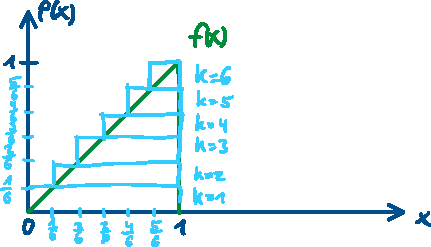
\includegraphics[width=0.80\textwidth]{Dateien/Hullreihe.pdf}
\end{center}
diese hat nun die Form $$\Phi_6(x)=\sum_{k=0}^{6-1}\frac{1}{6}\cdot 1_{[\frac{1}{6}k, 1]}$$ Lassen wir eine beliebige Anzahl $n$ an Quadern zu, gilt:
$$\Phi_n(x)=\sum_{k=0}^{n-1}\frac{1}{n}1_{[\frac{1}{n}k, 1]}$$
Der Inhalt ist dann
$$I(\Phi_n)=\frac{1}{n}\sum_{k=0}^{n-1} 1 -\frac{1}{n}k=\frac{1}{n}\sum_{k=0}^{n-1} 1 - \frac{1}{n^2}\sum_{k=0}^{n-1} k$$
$$=1-\frac{n-1}{2n}=\frac{1}{2}(1+\frac{1}{n})$$
Für $n\rightarrow \infty$ folgt:
$$I(\Phi_\infty)=\lim_{n\rightarrow\infty} \frac{1}{2}(1+\frac{1}{n})=\frac{1}{2}$$
Also dem Flächeninhalt unter der Funktion f!
\end{Beispiel}
\begin{Def}{$L^1$-Halbnorm}
Unter der \red{$L^1$-Halbnorm} von $f:\R^n\rightarrow\C\cup \{\infty\}$ versteht man das Infimum
$$||f||_1=\inf\{I(\Phi) |\mbox{ $\Phi$ Hüllreihe zu $f$} \}=\int |f|dx$$
\end{Def}
\begin{Satz}{Satz}{Eigenschaften einer Halbnorm}
Für die Funktionen $f_1, f_2: \R^n\rightarrow \C\cup\{\infty\}$ und ein $c\in\C$ gilt
\begin{enumerate}
\item $||c\cdot f||_1 = |c|\cdot ||f||_1$
\item $|f_1| \leq |f_2|  \implies ||f_1||_1 \leq ||f_2||_2$
\item $||\sum_{k=1}^\infty |f_k| ||_1\leq \sum_{k=1}^\infty ||f_k||_1$
\end{enumerate}
\end{Satz}
\newpage
\subsection{Lebesgue-Integral}
Mit den obigen theoretischen Werkzeug können wir nun endlich das Lebesgue-Integral definieren.
\begin{Def}{Lebesgue-Integral}
Eine Funktion $f:\R^n\rightarrow\C\cup\{\infty\}$ heißt \red{Lebesgue-integrierbar} über $\R^n$, wenn es eine Folge von Treppenfunktionen $\varphi_k$ gibt mit
$$\lim_{k\rightarrow \infty}||f-\varphi_k||_1=0$$
In diesem Fall schreiben wir das \red{Lebesgue-Integral}
$$\int fdx = \int f(x) d^nx = \int_{\R^n} f(x)dx = \lim_{k\rightarrow\infty} \varphi_k(x)dx\in\C$$
\end{Def}
\begin{Satz}{Satz}{Bedingte Gleichheit der Riemann und Lebesgue Integrale}
Sei $A=[a,b]$ ein kompaktes Intervall und $f$ eine über $A$ Riemann-integrierbare Funktion. Dann ist $f$ über $A$ Lebesgue-integrierbar und das Lebesgue-Integral und das Riemann-Integral sind gleich.
\end{Satz}
Der folgende zwei Sätze sind sehr wichtig in der Theorie der Gebietsintegrale. Im Skript stehen der kleiner und großer Satz von Fubini, wir schreiben hier aber die allgemeine Version aus T. Arens, also guckt euch auch das Skript nochmal an.
\begin{Satz}{Satz}{Kleiner Satz von Beppo Levi}
Sei $f:\R^n\rightarrow \R\cup \{\infty\}$ und sei $(\varphi_k)$ eine monoton wachsende oder fallende Folge von Treppenfunktionen, so dass
\begin{enumerate}[a)]
    \item $(\varphi_k)$ punktweise gegen $f$ konvergiert
    \item die Folge ($\int \varphi_k dx$) der Integrale der Treppenfunktionen beschränkt ist.
    Dann ist $f$ integrierbar und es gilt
    $$\int f dx=\lim_{k\rightarrow \infty}\int \varphi_k dx$$
\end{enumerate}
\end{Satz}
\begin{Satz}{Satz}{Satz von Fubini}
Sind $I\subseteq R^p$ und $J\subseteq R^q$ (möglicherweise unbeschränkte) Quader sowie $f\in L(Q)$ eine auf dem Quader $Q=I\times J \subseteq R^{p+q}$ integrierbare (oder mindestens stetig beschränkte) Funktion, so gibt es Funktionen $g\in L(I)$ und $h\in L(J)$ mit
$$g(x)=\int_J f(x,y) dy \mbox{ für fast alle $x\in I$}$$
$$h(y)=\int_I f(x,y)dx \mbox{ für fast alle $y\in J$}$$
Ferner ist 
$$\int_R f(x,y) d(x,y) = \int_I\int_J f(x,y) dy dx = \int_I g(x) dx$$
$$=\int_J\int_I f(x,y) dx dy = \int_J h(y) dy$$

\end{Satz}
\red{Wichtig!} Um den Satz von Fubini anwenden zu können, muss folgendes erwähnt werden:
\begin{itemize}
    \item $Q$ ist kompakt oder offen und beschränkt und
    \item $f$ ist stetig.
\end{itemize}
\begin{Beispiel}{Kompakte Kreissscheibe}
    Gegeben ist die kompakte Kreisscheibe:
    $$K=\overline{B_r(0)}=\{(x,y)\in\R^2| x^2+y^2\leq r^2\}$$
    Wir wollen nun das Integral
    $$\int_K 1 d(x,y)$$
    berechnen. Dazu stellen wir fest:
    \begin{enumerate}
        \item K ist kompakt
        \item $f(x,y)= 1$ ist stetig und beschränkt
        \item Die Menge $K_y$ lautet:
        $$K_y=\{x\in \R| (x,y)\in K\}=\{ x\in \R | x^2+y^2 \leq r^2\}$$
        $$= \{x\in \R | |x| \leq \sqrt{r^2-y^2}\}=[-\sqrt{r^2-y^2}, \sqrt{r^2-y^2}]$$
    \end{enumerate}
    Man erkennt leicht, dass $K_y\neq \emptyset$ für $y\in [-r, r]$. Somit erhalten wir:
    \begin{equation}
        F(y)=\begin{cases}\int_{K_y} 1dx & \mbox{ für $y\in [-1, 1]$} \\0 & \mbox{sonst}\end{cases}
    \end{equation}
    und damit nach dem Satz von Fubini:
    $$\int_K 1 d(x,y) = \int_\R F(y) dy = \int_{[-1,1]}[\int_{[-\sqrt{r^2-y^2}, \sqrt{r^2-y^2}]} 1dx]dy= \int_{-1}^{1} [\int_{-\sqrt{r^2-y^2}}^{\sqrt{r^2-y^2}} 1dx]dy=\pi r^2$$
    Eine nützliche Integrationsregel \red{$\int \sqrt{a^2-x^2}=\frac{1}{2}(a^2\sin^{-1}(\frac{x}{a})+x\sqrt{a^2-x^2})+c$}.
\end{Beispiel}
\begin{Beispiel}{Anwendung vom Satz von Fubini}
Wir wollen auch für eine kompliziertere Funktion, aber noch stets definiert auf einem Rechteck, die interierten Integrale berechnen. Dazu betrachten wir $R=(0,\frac{\pi}{2})\times (0,\frac{\pi}{2})$ und die Funktion $f:R\rightarrow \R$, die durch
$$f(x)=\sin(x_1+2x_2), \mbox{ $x=(x_1,x_2)\in R$}$$
gegeben ist. \\
Zunächst berechnen wir
$$\int_0^{\frac{\pi}{2}}\int_0^{\frac{\pi}{2}} \sin(x_1+2x_2)dx_2dx_1$$
$$=\int_0^{\frac{\pi}{2}}[-\frac{1}{2}\cos(x_1+2x_2)]^{\frac{\pi}{2}}_{x_2=0}dx_1$$
$$=\int_0^{\frac{\pi}{2}}(\frac{1}{2}\cos(x_1)-\frac{1}{2}\cos(x_1+\pi))dx_1$$
$$=\int_0^{\frac{\pi}{2}}\cos(x_1)dx_1 = 1$$
Nun vertauschen wir die Reihenfolge,
$$\int_0^{\frac{\pi}{2}}\int_0^{\frac{\pi}{2}} \sin(x_1+2x_2)dx_1dx_2$$
$$=\int_0^{\frac{\pi}{2}} [-\cos(x_1+2x_2)]^{\frac{\pi}{2}}_{x_1=0}dx_2$$
$$=\int_0^{\frac{\pi}{2}} (\cos(2x_2)-\cos(2x_2+\frac{\pi}{2}))dx_2$$
$$=[\frac{1}{2}\sin(2x_2)-\frac{1}{2}\sin(2x_2+\frac{\pi}{2})]_0^{\frac{\pi}{2}}$$
$$=\frac{1}{2}(\sin(\pi)-\sin(\frac{3\pi}{2})-\sin(0)+\sin(\frac{\pi}{2})) = 1$$
\end{Beispiel}
\begin{Beispiel}{Fubini ist nicht immer anwendbar}
\begin{center}
    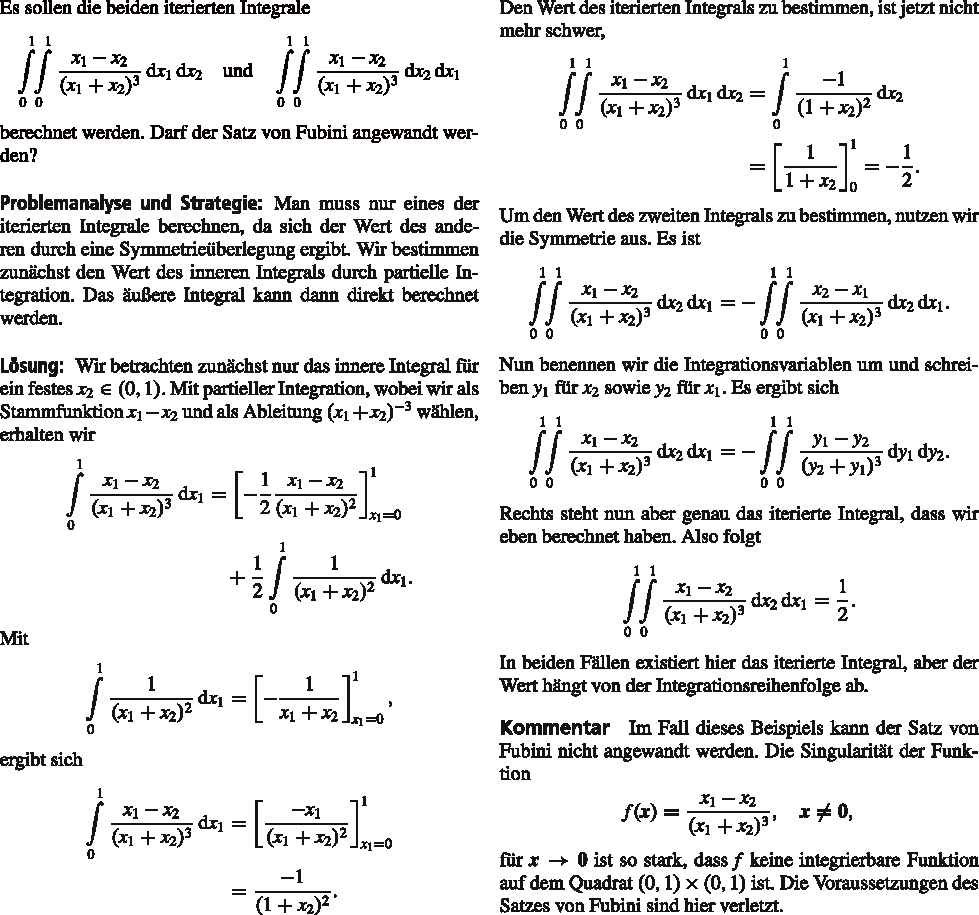
\includegraphics[width=\textwidth]{Dateien/Fubini.pdf}
\end{center}
\end{Beispiel}
\newpage
\subsection{Volumina und Nullmengen}

Wir beginnen dieses wichtige Thema mit sehr theoretischen Konzepten, die uns dann ermöglichen die Maßtheorie zu verstehen. So manche Begriffe werden in der Funktionalanalysis in MfP4 nochmal vorkommen.
\begin{Def}{Grundmenge und $\sigma$-Algebra}
Eine \red{Grundmenge} (auch Universum), $\Omega$, bezeichnet in der Mathematik eine Menge aus allen in einem bestimmten Zusammenhang betrachteten Objekten. \\
Eine Menge $\mathcal{A}$ von Teilmengen einer Grundmenge $\Omega$ heißt \red{$\sigma$-Algebra}, wenn
\begin{itemize}
    \item $\Omega \in \mathcal{A}$
    \item Für jede Menge $A\in \mathcal{A}$ gilt $\Omega / A\in \mathcal{A}$
    \item Abzählbare Vereinigungen von Mengen $A_i\in \mathcal{A}$ sind wieder in $\mathcal{A}$
\end{itemize}
\end{Def}
\begin{Beispiel}{Kleinste und größte $\sigma$-Algebra}
Für jede beliebige Menge $\Omega$ ist $\{\emptyset, \Omega\}$ die kleinste und die Potenzmenge $P(\Omega)$ die größtmögliche $\sigma$-Algebra mit $\Omega$ als Grundmenge.
\end{Beispiel}
\begin{Def}{Maß}
Sei $\mathcal{A}$ eine $\sigma$-Algebra. Eine Funktion $\mu: \mathcal{A}\rightarrow[0,\infty]$ heißŧ ein \red{Maß} auf $\mathcal{A}$, wenn
\begin{itemize}
    \item $\mu(\emptyset)=0$,
    \item $\sigma$-Additivität, also $\mu(\cup_{n=1}^\infty A_n)=\sum_{n=1}^\infty \mu(A_n)$.
\end{itemize}
Außerdem wird das Tripel $(\Omega, \mathcal{A}, \mu)$ \red{Maßraum} gennant.
\end{Def}
\begin{Beispiel}{Borelsche $\sigma$-Algebra}
Die \red{borelsche $\sigma$-Algebra} ist eine $\sigma$-Algebra, die alle Mengen enthält, denen man naiverweise ein Volumen oder eine Wahrscheinlichkeit zuordnen will, schließt aber Negativresultate aus. \\
Bezüglich der borelschen $\sigma$-Algebra sind alle stetigen Funktionen immer messbar.
\end{Beispiel}
\begin{Def}{$\sigma$-Kompaktheit}
    Eine Menge $A\subseteq \R^n$ heißt \red{$\sigma$-kompakt}, wenn sie eine Vereinigung abzählbar vieler kompakter Menger ist.
\end{Def}
Nun kommt eine sehr wichtige Definition.
\begin{Def}{Lebesgue-Messbarkeit}
Eine Menge $A\subseteq \R^n$, falls die konstante Funktion über $A$ integrierbar ist.
$$v(A)=v_n(A)=\int_A 1dx$$
\end{Def}
\begin{Def}{Figur und Ausschöpfung}
Eine Vereinigung endlich vieler Quader $Q_i\subseteq \R^n$ der Form $A=Q_1\cup Q_2 \cup \dots \cup Q_s$ heißt \red{Figur}. \\
Eine \red{Ausschöpfung} von $A$ ist eine aufsteigende Folge von Teilmengen $A_1\subseteq A_2 \subseteq \cdots \subseteq A$.
\end{Def}
\begin{Beispiel}{Volumina von Kegeln}
Wir sollen das Volumen des Kegels
$$K=\{(x,y)\in \R^n | y\in [0,h], x\in (1-\frac{y}{h})B\}$$
mit kompakter Basis (das ist die Fläche des Kegels ganz unten) $B\subseteq \R^{n-1}$ und Höhe $h>0$ bestimmen. Da wir in 3D arbeiten ist unser $n=3$.
$$v_n(K)=\int_0^k v_{n-1} ((1-\frac{y}{h})B)dy$$
An dieser Stelle ist es wichtig die \red{Streckungsformel} zu kennen
\blue{$$\int_{\R^n} (s_1x_1, \dots, s_nx_n)dx=s_1^{-1}s_2^{-1}\dots s_n^{-1}\int_{\R^n}f(x)dx$$}
$$v_n(K)=\int_0^h v_{n-1}(B)(1-\frac{y}{h})^{n-1}dy=B\int_0^h (1-\frac{y}{h})^2 dy=\frac{B\cdot h}{3}$$
\end{Beispiel}
Und nun eins der wichtigsten Definitionen im MfP3.
\begin{Def}{Nullmenge}
Eine Teilmenge $N\subseteq \R^n$ heißt Lebesgue-Nullmenge, wenn sie eine der beiden folgenden Bedingungen erfüllt:
\begin{itemize}
    \item $N$ ist messbar mit $v_n(N)=0$.
    \item Für die charakteristische Funktion gilt $||1_{N}||_1=0$.
\end{itemize}
\end{Def}
\begin{Beispiel}{Nullmengen}
Überlegen Sie sich einige Beispiele für Nullmengen im $\R^2$ und im $\R^3$. \\ \\
In jedem Fall sind isolierte Punkte und abzählbare Vereinigungen von isolierten Punkten wie im eindimensionalen Nullmengen. Das bedeutet etwa, dass $\Q^2\subset \R^2$ oder $\Q^3 \subset \R^3$ Nullmengen sind. \\ \\
Der Rand eines Quaders, im zweidimensionalen also der Rand eines Rechtecks, ist ebenfalls eine Nullmenge. Dasselbe gilt für abzählbare Vereinigungen solcher Ränder. \\ \\
Als letztes Beispiel im $\R^2$ sei der Graph einer Funktion $f:\R\rightarrow \R$ gennant.
\end{Beispiel}
\begin{Def}{Fast überall}
Sei $E(x)$ eine Eigenschaft, sodass wir für $\forall x \in \R^n$ wissen, ob die Eigenschaft $E(x)$ erfüllt ist. Wir sagen, dass $E(x)$ \red{fast überall} gilt, wenn die Menge aller Punkte, wo $E(x)$ nicht gilt, eine Nullmenge ist.
\end{Def}
\begin{Beispiel}{Fast überall konstante Funktion}
Sei $f(x)=\begin{cases}42 \mbox{ wenn $x\neq \infty$} \\
\infty \mbox{ wenn $x=\infty$}\end{cases}$. Die Funktion $f(x)$ ist fast überall konstant, außer in einer Nullmenge (also in der Unendlichkeit). 
\end{Beispiel}
Es ist auch nützlich sich zu merken, dass wenn $||f||_1=0$, dann $N=\{ x\in \R^n | f(x)\neq 0\}$ eine nullmenge ist.
\begin{Satz}{Satz}{Modifikationssatz}
Seien $f,g:\R^n\rightarrow \C$ zwei Funktionen, die fast überall gleich sind. Wenn $f$ integrierbar ist, dann ist auch $g$ integrierbar und es gilt $\int f = \int g$.
\end{Satz}
\begin{Satz}{Lemma}{Geometrische Charakterisierung von Nullmengen}
    Ist $N$ eine Nullmenge, so gibt es zu jedem $\epsilon>0$ eine messbare offene Menge $U$ mit $N\subseteq U$ und $v(U)<\epsilon$. \\
    Eine Menge $N\subseteq \R^n$ ist genau dann eine Nullmenge, wenn es zu jedem $\epsilon>0$ abzählbar viele Quader $Q_1, Q_2, ..., Q_n$ gibt, sodass
    $$N\subseteq \bigcup_{k=1}^{\infty}Q_k \mbox{ und }\sum_{k=1}^\infty v(Q_k)>\epsilon$$
\end{Satz}
Eine nützliche, aber nicht so wichtige Eigenschaft ist, dass wenn $f$ integrierbar ist, dann auch $f(x-a)$ integrierbar ist, wenn $a$ in der Definitionsmenge ist.
\newpage
\subsection{Konvergenzsätze}
Zuerst wollen wir uns an die punktweise und gleichmäßige Kovergenz aus MfP2 erinnern.
\begin{Def}
{Gleichmäßige Konvergenz}
Sind $(X,d_X)$ und $(Y,d_Y)$ metrische Räume und $(f_n:X\to Y)_{n\in\mathbb{N}}$ eine Folge von Abbildungen.\\
Wir sagen, dass $f$ genau dann \red{gleichmäßig} gegen eine Grenzfunktion $f$ \red{konvergiert}, wenn es für alle $\epsilon>0$ ein $N=N(\epsilon)\in\mathbb{N}$ gibt, sodass
\begin{equation*}
    d_Y(f_n(x),f(x))<\epsilon\quad \forall n\geq N\land \forall x\in X.
\end{equation*}
\end{Def}
\begin{Def}
{Punktweise Konvergenz}
Eine Folge $(f_n)$ von Abbildungen \red{konvergiert punktweise} gegen eine Abbildung $f$, falls $\lim_{n\to\infty}f_n(x)=f(x)\,\forall x\in X$.
\end{Def}
\begin{Beispiel}
    {Gleichmäßige Konvergenz}
    Wir betrachten die Funktionenfolge
    \begin{equation*}
        f_n(x)=\sqrt{\vert x \vert^2 + \frac{1}{n^2}} \qquad x \in \mathbb{R}.
    \end{equation*}
    Konvergiert diese Folge gleichmäßig gegen eine Grenzfunktion, sagen wir $f(x)=\vert x \vert$? In weiser Voraussicht und um die weitere Rechnung plausibel zu machen, schauen wir uns zunächst die folgende Ungleichung an: 
    \begin{equation*}
        \sqrt{a+b} \leq \sqrt{a+b+2\sqrt{ab}} = \sqrt{(\sqrt{a}+\sqrt{b})^2}=\sqrt{a}+\sqrt{b}.
    \end{equation*} \\
    
    Damit können wir nun recht schnell nachprüfen:
    \begin{align*}
        \forall \epsilon > 0 \,\exists N\in\mathbb{N}\, &\forall x\in D_f \,\forall n\geq N: \\
            &\vert f_n(x)-f(x) \vert = \bigl| \sqrt{\vert x \vert^2 + \frac{1}{n^2}} - \vert x \vert \bigr| \leq \bigl| \vert x \vert + \frac{1}{n} - \vert x \vert \bigr| = \frac{1}{n} \leq \frac{1}{N} < \epsilon
    \end{align*}
    Das Kriterium ist also erfüllt und die Funktion damit gleichmäßig konvergent (und daher auch automatisch punktweise konvergent), da wir die $x$-Abhängigkeit in der Abschätzung losgeworden sind.
\end{Beispiel}
Ebenso ein Beispiel, um uns auf die Quotientenvektorräume aus MfP2 zu erinnern.
\begin{Beispiel}{Quotientenvektorraum}
    Sei $V=\R^4$ und $U=span\{(1,1,0,0)^T, (0,1,-1,0)^T\}\subseteq V$ ein Untervektorraum. Wir sollen zeigen, dass im Quotientenvektorraum $U/V$ gilt
    $$[\begin{pmatrix}
        1 \\
        0 \\
        1 \\
        2 \\
    \end{pmatrix}]=[\begin{pmatrix}
        3 \\
        1 \\
        2 \\
        2 \\
    \end{pmatrix}] \mbox{ und }[\begin{pmatrix}
        1 \\
        0 \\
        1 \\
        0 \\
    \end{pmatrix}]\neq[\begin{pmatrix}
        1 \\
        0 \\
        0 \\
        0 \\
    \end{pmatrix}]$$
    Dabei bezeichnet [$v$] die Äquvialenzklasse von $v\inV$ von $V/U$. \\
    Ein Quotientenvektorraum besteht aus allen Vektoren $a,b\in V$ für die gilt $a+b\in U$.
    $$\begin{pmatrix}
        1 \\
        0 \\
        1 \\
        2 \\
    \end{pmatrix}+\begin{pmatrix}
        3 \\
        1 \\
        2 \\
        2 \\
    \end{pmatrix}=\begin{pmatrix}
        4 \\
        1 \\
        3 \\
        0 \\
    \end{pmatrix}$$
    Wir können nun den Vektor $\begin{pmatrix}
        4 \\
        1 \\
        3 \\
        0 \\
    \end{pmatrix}$ mit den Basisvektoren von $U$ darstellen
    $$\begin{pmatrix}
        4 \\
        1 \\
        3 \\
        0 \\
    \end{pmatrix}= a \begin{pmatrix}
        1 \\
        1 \\
        0 \\
        0 \\
    \end{pmatrix}+b\begin{pmatrix}
        0 \\
        1 \\
        -1 \\
        0 \\
    \end{pmatrix}$$
    Wenn wir $a=4$ und $b=1$ setzen, dann wird das Ungleichungssystem gelöst. Also stimmt die erste Äquivalenzklasse. Nun gucken wir uns das für die anderen zwei Vektoren an
    $$\begin{pmatrix}
        1 \\
        0 \\
        1 \\
        0 \\
    \end{pmatrix}+\begin{pmatrix}
        1 \\
        0 \\
        0 \\
        0 \\
    \end{pmatrix}=\begin{pmatrix}
        2 \\
        0 \\
        1 \\
        0 \\
    \end{pmatrix} \mbox{,     } \begin{pmatrix}
        2 \\
        0 \\
        1 \\
        0 \\
    \end{pmatrix}=a \begin{pmatrix}
        1 \\
        1 \\
        0 \\
        0 \\
    \end{pmatrix}+b\begin{pmatrix}
        0 \\
        1 \\
        -1 \\
        0 \\
    \end{pmatrix}$$
    Und wir merken schon, dass es keine $a$ und $b$ gibt, sodass das Gleichungssystem gelöst werden kann, daher gehören die letzten zwei Vektoren nicht zu der Äquvivalenzklasse.
\end{Beispiel}
Nun kommen wir zu sehr wichtigen Sätzen.
\begin{Satz}{Theorem}{Satz von Riesz-Fischer}
    Vorausgesetzt $f_k$ ist eine $\mathcal{L}^1$-Cauchy-Folge integrierbarer Funktionen, dann \begin{itemize}
        \item existiert $f\in \mathcal{L}^1(\R^n)$ mit $\lim_{k\rightarrow \infty}f_k = f$ mit $\int f dx = \lim_{k\rightarrow \infty}\int f_k dx$ und
        \item $(f_k)$ konvergiert punktweise gegen $f$.
    \end{itemize}
    Somit ist $\mathcal{L}^1(\R^n)$ ein Banachraum. Die \red{Vertauschbarkeit} von Integral und Limes folgt grob aus der Konvergenz bzgl. der $\mathcal{L}^1$-Halbnorm.
\end{Satz}
Beachtet, dass der $\mathcal{L}^1$- Grenzwert nicht eindeutig ist, aber es kann sein, dass sich die Grenzwerte nur auf eine Nullmenge unterscheiden.
\begin{Satz}{Satz}{Satz von Beppo-Levi von der monotonen Konvergenz}
    Voraussetzungen:
    \begin{itemize}
        \item $f_k:\R^n\rightarrow \R \cup \{ \infty\}$ ist monoton wachsende/fallende Folge integrierbarer Funktionen
        \item $f_k$ konvergiere punktweise gegen $f(x)=\lim_{k\rightarrow \infty} f_k(x)$
        \item Die Folge $\int f_k dx$ der Integrale ist beschränkt.
    \end{itemize}
    Dann folgt, dass $f$ integrierbar ist und dass $\lim_{k\rightarrow \infty} \int f_k dx=\int f dx$
\end{Satz}
\begin{Satz}{Satz}{Satz von Lebesgue von der majorisitierten Konvergenz}
    Voraussetzungen:
    \begin{itemize}
        \item $f_k:\R^n\rightarrow \C \cup \{ \infty\}$ ist eine Folge integrierbaren Funktionen
        \item $f_k$ konvergiert fast überall punktweise gegen eine Funktion $f$
        \item Es gibt eine integrierbare Majorante $F$ mit $|f_k|\leq F$ für $\forall k$.
    \end{itemize}
    Dann folgt, dass $f$ integrierbar ist und dass $\lim_{k\rightarrow \infty} \int f_k dx = \int f dx$
\end{Satz}
\begin{Beispiel}{Satz von integrierbaren Majoranten angewandt}
    Wir betrachten die Funktion
    $$\delta_n(x)=\begin{cases}
        xn^2 & 0\leq x< \frac{1}{n} \\
        2n-xn^2 & \frac{1}{n} \leq x \leq \frac{2}{n} \\
        0 & \mbox{sonst}
    \end{cases}$$
    Die Funktionenfolge ist unbeschränkt wie wir gesehen haben, da
    $$\max_{x\in\R} \delta_n(x)=n$$
    Es gibt also keine integrierbare Majorante und somit ist nicht sichergestellt, dass Integral und Limes vertauschen zu können. Tatsächlich gilt:
    $$\lim_{n\rightarrow \infty} \int_\R \delta_n(x) dx = 1 \mbox{ und } \int_\R \delta(x)dx = 0$$
\end{Beispiel}
\begin{Beispiel}{Und noch ein Beispiel}
Wir betrachten das Integral
$$\lim_{n\rightarrow \infty}\int_0^\infty (1+\frac{x}{n})^n\cos(\frac{x}{n})e^{-2x}dx$$
Die Funktionenfolge, die wir dafür untersuchen müssen, ist
$$f_n(x)=(1+\frac{x}{n})^2n\cos(\frac{x}{n})e^{-2x}$$
Aus MfP1 wissen wir, dass
$$(1+\frac{x}{n})^n \mbox{ wächst monoton, } \lim_{n\rightarrow \infty}(1+\frac{x}{n})^n=e^x$$
wir gehen nun schrittweise vor: \begin{enumerate}
    \item \blue{$f_n(x)$ ist eine Folge integrierbarer Funktionen, denn} \\
    \begin{itemize}
        \item $f_n(x)$ ist steig und daher lokal-integrierbar über die $\sigma$-kompakte Menge $(0,\infty)$.
        \item $f_n(x)$ hat die über $(0,\infty)$ integrierbare Majorante
        $$|(1+\frac{x}{n})^n\cos(\frac{x}{n})e^{-2x}|<e^xe^{-2x}=e^{-x}$$
        denn $$\int_0^\infty e^{-x}= 1$$
        \item $f_n(x)$ ist damit auch über $(0,\infty)$ integrierbar.
    \end{itemize}
    \item \blue{$f_n(x)$ konvergiert fast überall punktweise} \\
    Es gilt $$\lim_{n\rightarrow \infty} (1+\frac{x}{n})^n\cos(\frac{x}{n})e^{-2x}$$
    $$=e^{-2x}\lim_{n\rightarrow \infty} (1+\frac{x}{n})^n \cdot \lim_{n\rightarrow \infty} \cos(\frac{x}{n})$$
    $$=e^{-2x}\cdot e^x=e^{-x}$$
    Die Grenzfunktion ist also $f(x)=e^{-x}$.
    \item \blue{$f_n(x)$ hat eine integrierbare Majorante} \\
    Die haben wir mit $f(x)=e^{-x}$ schon gefunden.
\end{enumerate}
Nun können wir den Satz von Lebesgue von der majorisierten Konvergenz anwenden und Integral und Limes vertauschen:
$$\lim_{n\rightarrow \infty} \int_0^\infty (1+\frac{x}{n})^n\cos(\frac{x}{n})e^{-2x}dx = \int_0^\infty e^{-x} = 1$$
\end{Beispiel}
\newpage
\subsection{Parameterabhängige Integrale}
Die Vertauschbarkeit von Integral und Limes führt zu weiteren, sehr praktischen Sätzen.
\begin{Satz}{Satz}{Verallgemeineter Hauptsatz der Differential- und Integralrechnung}
Voraussetzungen:
\begin{itemize}
    \item $f$ ist differenzierbar auf dem kompakten Intervall $[x_0, x]$.
    \item Die Ableitung von $f$ ist beschränkt.
\end{itemize}
Daraus folgt, dass $f'$ Lebesgue-integrierbar ist über $[x_0, x]$ und dass $$f(x)-f(x_0)=\int_{[x_0, x]} f'(t)dt$$.
\end{Satz}
\begin{Satz}{Satz}{Stetigkeitssatz}
    Voraussetzungen:
    \begin{itemize}
        \item Sei $X$ ein metrischer Raum und $T\subseteq \R^p$
        \item $f:X\times T\rightarrow \C, (x,t)\longmapsto f(x,t)$ ist für feste $x$ über $T$ integrierbar
        \item Für feste $t$ ist die Funktion $x\longmapsto f(x,t)$ stetig
        \item Es gibt eine integrierbare Majorante $\Phi: T\rightarrow \R$, sodass $|f(x,t)|\leq \Phi(t)$ für $\forall (x,t)\in X\times T$.
    \end{itemize}
    Daraus folgt, dass $F(x)=\int_T f(x,t)dt$ auf $X$ stetig ist.
\end{Satz}
\begin{Satz}{Satz}{Differentiationssatz}
        Voraussetzungen:
    \begin{itemize}
        \item Sei $X\subseteq \R^n$ und $T\subseteq \R^p$
        \item $f: X\times T\rightarrow \C$, $(x,t)\rightarrow f(x,t)$ ist für feste $x$ über $T$ integrierbar
        \item Für feste $t$ ist die Funktion $x\longmapsto f(x,t)$ stetig diff'bar
        \item Es gibt eine intergierbare Majorante $\Phi:T\rightarrow \R$ mit
        $$|\frac{\partial f}{\partial v_\mu}(x,t)|\leq \Phi(t)\mbox{ für }\forall (x,t)\in X\times T\mbox{ für }\mu = 1,...,n$$
    \end{itemize}
    Daraus folgt, dass
    \begin{itemize}
        \item $F(x)=\int_T f(x,t)dt$ ist stetig diff'bar,
        \item $t\mapsto\frac{\partial}{\partial x_p}f(x,t)$ ist für jedes $x$ integrierbar und
        \item es gilt $\frac{\partial}{\partial x_\mu}\int_T f(x,t)dt=\int_T \frac{\partial}{\partial x_\mu} (x,t) dt$.
    \end{itemize}
\end{Satz}
\begin{Beispiel}{Fourier-Transformation}
Die \red{Fourier-Transformierte} ist definiert durch:
$$\hat{f}(x)=\frac{1}{\sqrt{2\pi}}\int_{\R} f(t)e^{-ixt}dt$$
wobei $f$ eine integrierbare Funktion ist. Wir überprüfen $\hat{f}(x)$ zunächst auf Stetigkeit: \\
\begin{enumerate}
    \item $t\mapsto f(t)e^{-ixt}$ ist für feste $x$ über $\R$ integrierbar? \\
    \blue{Ja, denn $|f| = |e^{-ixt}f(t)|$ ist eine integrierbare Majorante.}\\
    \item Für feste $t$ ist $x\mapsto f(t)e^{-ixt}$ stetig?\\
    \blue{Ja klar! $f(t)$ ist fest und $e^z$ ist immer stetig.} \\
    \item Gibt es eine integrierbare Majorante? \\
    \blue{Ja, nämlich $\Phi(t)=|f(t)|$.}\\
\end{enumerate}
Somit ist $\hat{f}$ tatsächlich stetig. Wir setzten nun $f(t)=e^{-\frac{t^2}{2}}\Rightarrow \hat{f}(x)=\frac{1}{\sqrt{2\pi}}\int_{\R} e^{-\frac{t^2}{2}}e^{-ixt}dt$.
Zunächst formen wir den Exponenten etwas um: \\
$$-\frac{t^2}{2}-ixt=-\frac{1}{2}(t+ix)^2-\frac{x^2}{2}$$
So erhalten wir das Integral:
$$\hat{f}(x)=\frac{1}{\sqrt{2\pi}}e^{-\frac{x^2}{2}}\int_{\R} e^{-\frac{1}{2}(t+ix)^2}dt$$
Nun können wir den Differentationssatz anwenden. Dazu schränken wir ohne Beschränkung der Allgemeinheit den Definitionsbereich von $x$ auf das offene Intervall $(-a,a)$ ein.
$$F_a(x)=\int_{\R}e^{-\frac{1}{2}(t+ix)^2}dt \quad x\in(-a,a)\quad a\in\R$$
\begin{enumerate}
    \item Ist $t\mapsto e^{-\frac{1}{2}(t+ix)^2}$ integrierbar? \\
    \blue{Wir finden die integrierbare Majorante $|e^{-\frac{1}{2}(t+ix)^2}|=|e^{-\frac{1}{2}t^2+\frac{1}{2}x^2-ixt}| =e^{\frac{1}{2}x}e^{-\frac{1}{2}t^2}=\Phi(t)$} \\
    \item Ist $x\mapsto e^{-\frac{1}{2}(t+ix)^2}$ stetig differenzierbar?\\
    \blue{ja klar! Es gilt $\frac{\partial}{\partial x}e^{-\frac{1}{2}(t+ix)^2}=-i(t+ix)e^{-\frac{1}{2}(t+ix)^2}$} \\
    \item Gibt es eine integrierbare Majorante von $\frac{\partial}{\partial x}e^{-\frac{1}{2}(t+ix)^2}$? \\
    \blue{$|\frac{\partial}{\partial x}e^{-\frac{1}{2}(t+ix)^2}|\leq (|t|+a)e^{-\frac{1}{2}t^2}e^{\frac{1}{2}a^2}$} \\
\end{enumerate}
Wir können nun den Differentationssatz anwenden:
\blue{$$\frac{dF_a}{x}=\int_{\R}\frac{\partial}{\partial x} e^{-\frac{1}{2}(t+ix)^2}dt$$
$$=\lim_{b\rightarrow \infty} ie^{-\frac{1}{2}(t+ix)^2}|_{-b}^{b}=0$$}
Bisher haben wir uns nur auf das Intervall $x\in(-a,a)$ eingeschränkt. Wir können aber problemlos schreiben:
\blue{$$\frac{\partial F}{\partial x}=\lim_{a\rightarrow \infty} \frac{\partial F_a}{\partial x}=\lim_{a\rightarrow \infty} 0 = 0$$}
Somit ist $F(x)=F(0)=const.$ und wir können rechnen:
\blue{$$F(x)=F(0)=\int_{\R}e^{-\frac{1}{2}t^2}dt=\sqrt{2\pi} \quad \mbox{(Gauß-Integral)}$$ }
Jetzt können wir die Fourier-Transformierte ausrechnen:
\blue{$$\hat{f}(x)=\frac{1}{\sqrt{2\pi}}e^{-\frac{1}{2}^2}f(x)=e^{-\frac{1}{2}x^2}$$}
Also sind $\hat{f}(x)$ und $f(t)$ die gleichen Funktionen! Dies ist eine ganz wichtige Feststellung, die z.B. bei der Unschärferelation der Quantenmechanik wichtig wird.
\end{Beispiel}
\newpage
Aus all diesen Sätzen kommt nun der Höhepunkt der Integrationstheorie. Die folgenden zwei Sätze sind von enormer bedeutung in der Physik, also merkt sie euch. 
\begin{Satz}{Satz}{Satz von Tonelli}
    Vorausgesetzt $f:\R^p\times \R^q \rightarrow \C$ ist fast überall stetig oder lokal integrierbar. Dann gilt die folgende Äquivalenz
    $$\int_{\R^q}(\int_{\R^p} |f(x,y)|dx)dy \quad\mbox{oder}\quad\int_{\R^p}(\int_{\R^q} |f(x,y)|dy)dx\mbox{ existiert} $$
    $$\iff \mbox{$f$ ist über $\R^p\times\R^q$ integrierbar}$$
\end{Satz}
\begin{Satz}{Satz}{Transformationssatz}
Seien $B,D\in\R^n$ offen und $\psi: B\rightarrow D$ ein Diffeomorphismus. Eine Funktion $f: D\rightarrow \R$ ist genau dann über $D$ integrierbar, wenn $f(\psi(x))\cdot|\det(d\psi)|$ über $B$ integrierbar ist, und es gilt:
$$\int_D f(x) dx = \int_B f(\psi(y))\cdot|\det(d\psi(y))|dy$$
\end{Satz}
Zur Erinnerung die definition der allgemeinen linearen Gruppe: $$GL(n,\R)=\{A\in \mbox{Mat}(n,\R)| \det(A)\neq0\}$$
Außerdem nicht vergessen, dass der Betrag der Determinante einer Matrix das gerichtete Volumen eines Parallelepipeds darstellt.
\begin{Beispiel}{Präsenzaufgabe 1 aus dem Übungsblatt 7}
    Wir mussten, für $a,b>0$, den Flächeninhalt einer Ellipse mit dem Transformationssatz bestimmen.
    $$E=\{(x,y)| \frac{x^2}{a^2}+\frac{y^2}{b^2} \leq 1\}$$
    Da die Kugel als $B_1(0)=\{(x,y)| x^2+y^2 \leq 1\}$ definiert ist, ist es sinnvoll die Abbildung $\psi(x,y)=(\frac{x}{a}, \frac{y}{b})$ zu wählen (dies ist auch ein \blue{Diffeomorphismus}).
    $$d\psi(x,y)=\begin{pmatrix}
        \frac{1}{a} & 0 \\
        0 & \frac{1}{b}
    \end{pmatrix}$$
    $$\det(d\psi(x,y))=\frac{1}{ab}$$
    Wir wissen, dass $v(B_1(0))=\int_{B_1(0)} 1dx = \pi$ also können wir die Gleichung aufstellen:
    $$\int_{B_1(0)}1 dx = \int_E \frac{1}{ab}\cdot 1 dy$$
    $$\int_{B_1(0)}1 dx = \frac{1}{ab}\int_E 1 dy$$
    $$\int_E 1 dy = ab\pi$$
\end{Beispiel}
\begin{Beispiel}{Bestimmung eines uneigentlichen 3D-Integrals}
    \begin{center}
    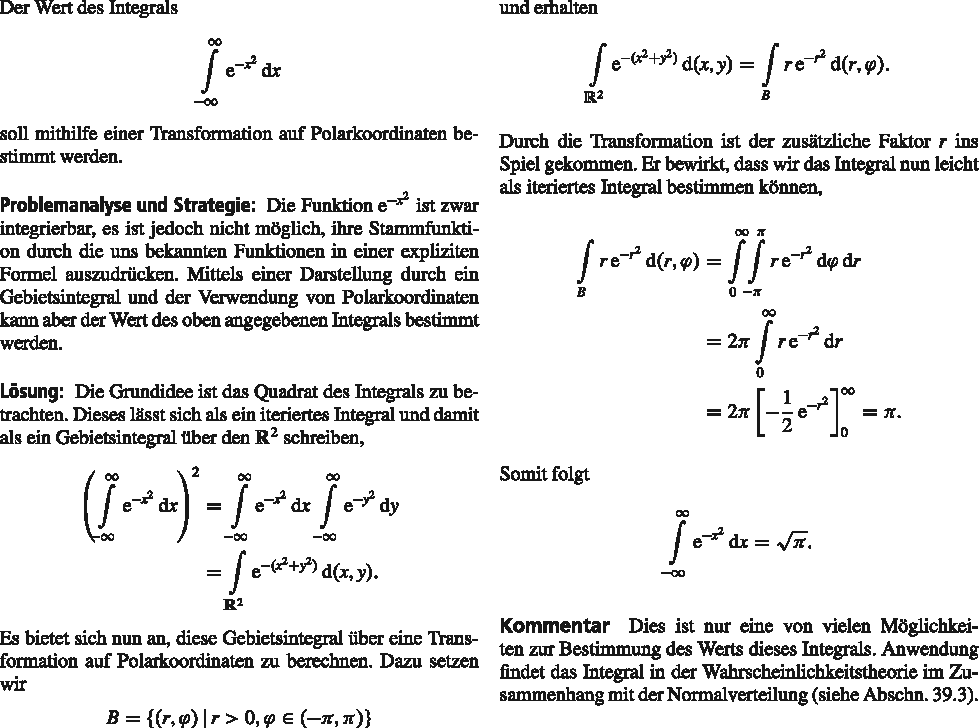
\includegraphics[width=0.95\textwidth]{Dateien/Uneigentlich.pdf}

\end{center}
\end{Beispiel}
\begin{Beispiel}{Transformationssatz im Einsatz}
Das Integral $$\int_D \sqrt{x_1}x_2 dx$$ mit $$D=\{ x\ \in\R^2 | x_1, x_2 >0, \sqrt{x_1}<x_2<2\sqrt{x_1}, \frac{1}{x_1}<x_2<\frac{2}{x_1}\}$$
soll berechnet werden. Das Gebiet $D$ ist auf dem Bild zu sehen. \\
            \begin{center}
    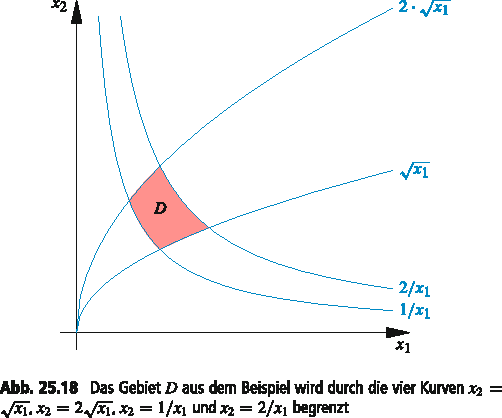
\includegraphics[width=0.50\textwidth]{Dateien/Trafo.pdf}
\end{center}
Um eine geeignete Transformation zu finden, betrachten wir die Bedingungen in der Definition von $D$ genauer. Sie lassen sich umschreiben zu
$$1<\frac{x_2}{\sqrt{x_1}}<2 \mbox{ und } 1<x_1x_2<2$$
Es liegt daher nahe, als neue Koordinaten $u_1=x_1x_2$ und $u_2=\frac{x_2}{\sqrt{x_1}}$ zu wählen. Umgekehrt hat man dann
$$x=\psi(u)=\begin{pmatrix}
    u_1^{\frac{2}{3}} & u_2^{-\frac{2}{3}} \\
    u_1^{\frac{1}{3}} & u_2^{\frac{2}{3}}
\end{pmatrix} \mbox{, $1<u_1, u_2 < 2$.}$$
Da man die Darstellung von $u$ durch $x$ und umgekehrt äquivalent in einander umformen kann, ist diese Transformation bijektiv. Als Funktionaldeterminante ergibt sich
$$\det \psi '(u)=\det \begin{pmatrix}
    \frac{2}{3}u_1^{{-\frac{1}{3}}}u_2^{-{\frac{2}{3}}} & -\frac{2}{3}u_1^{\frac{2}{3}}u_2^{-{\frac{5}{3}}} \\
    \frac{1}{3}u_1^{-{\frac{2}{3}}}u_2^{\frac{2}{3}} & {\frac{2}{3}}u_1^{\frac{1}{3}}u_2^{-\frac{1}{3}}
\end{pmatrix}=\frac{4}{9}u_2^{-1}+\frac{2}{9}u_2^{-1}=\frac{2}{3u_2}$$
Die Determinante ist daher stets positiv. Wir können nun die Transformationsformel anwenden und erhalten mit $B=(1,2)\times(1,2)$.
$$\int_D \sqrt{x_1}x_2 dx = \int_B u_1^{\frac{1}{3}}u_2^{-\frac{1}{3}}u_1^{\frac{1}{3}}u_2^{\frac{2}{3}}\frac{2}{3u_2}du$$
$$=\frac{2}{3}\int_1^2 \int_1^2 u_1^{\frac{2}{3}}u_2^{-\frac{2}{3}}du_1du_2$$
$$=\frac{2}{5}(\sqrt[3]{32}-1)\int_1^2 u_2^{-{\frac{2}{3}}}du_2=\frac{6}{5}(\sqrt[3]{32}-1)(\sqrt[3]{2}-1)$$
$$=\frac{6}{5}(5-\sqrt[3]{32}-\sqrt[3]{2})$$

\end{Beispiel}
\newpage
\subsection{Exkurs: Wichtige Koordinatensysteme}
Dieses Thema ist euch allen schon aus der Physik 2 bekannt und könnt es überspringen, aber guck euch die Beispiele zur Erinnerung vor der Klausur nochmal an. \\
Für das \red{Polarkoordinatensystem} gelten die folgenden Gleichungen:
$$x_1=r\cos(\varphi)$$
$$x_2=r\sin(\varphi)$$
$$\Phi(r, \varphi) = \begin{pmatrix}
    r\cos(\varphi) \\
    r\sin(\varphi)
\end{pmatrix}$$
\begin{Def}{Integration mit Polarkoordinaten}
Ist $D\subseteq \R^2, f\in L(D)$ und $B$ die Beschreibung von $D$ durch Polarkoordinaten, so gilt
$$\int_D f(x_1,x_2)d(x_1,x_2) = \int_B f(r\cos(\varphi), r\sin(\varphi))rd(r, \varphi)$$
\end{Def}
\begin{Beispiel}{Integration mit Polarkoordinaten}
Berechnen wir das Integral $$\int_D x(x^2+y)d(x,y)$$
mit $D=\{ x\in \R^2 | x>0, 1<x^2+y^2<4\}$. Wir wollen dies mit Polarkoordinaten ausrechnen. Wir drücken $D$ aus durch
$$D=\{ (r\cos(\varphi), r\sin(\varphi))^T \in \R^2 | -\frac{\pi}{2}<\varphi<\frac{\pi}{2}, 1<r<2 \}$$
Das Gebiet $B$ aus dem Transformationssatz ist also genau das Rechteck
$$B=\{ (r,\varphi) \in \R^2 | -\frac{\pi}{2}<\varphi<\frac{\pi}{2}, 1<r<2 \}$$
Damit ergibt sich:
$$\int_D x(x^2+y)d(x,y)=\int_B (r^3\cos^3(\varphi)+r^2\cos(\varphi)\sin(\varphi))rd(r,\varphi)$$
$$=\int_1^2\int_{-\frac{\pi}{2}}^{\frac{\pi}{2}} (r^4\cos^3(\varphi)+r^3\cos(\varphi)\sin(\varphi)) d\varphi dr$$
$$=\int_1^2 [\frac{r^4}{3}\sin(\varphi)\cos^2(\varphi)+\frac{2r^4}{3}\sin(\varphi)+\frac{r^3}{2}\sin^2(\varphi)_{-\frac{\pi}{2}}]^{\frac{\pi}{2}}dr$$
$$=\int_1^2 \frac{4}{3}r^4 dr = [\frac{4}{15}r^5]_1^2=\frac{124}{15}$$
\end{Beispiel}

Für das \red{Zylinderkoordinatensystem} gelten die folgenden Gleichungen:
$$x_1=\rho\cos(\varphi)$$
$$x_2=\rho \sin(\varphi)$$
$$x_3=z$$
$$\Phi(\rho, \varphi, z)=\begin{pmatrix}
    \rho \cos(\varphi) \\
    \rho \sin(\varphi) \\
    z
\end{pmatrix}$$
\begin{Def}{Integration mit Zylinderkoordinaten}
Ist $D\subseteq \R^3, f\in L(D)$ und $B$ die Beschreibung von $D$ durch Polarkoordinaten, so gilt
$$\int_D f(x_1,x_2,x_3)d(x_1,x_2,x_3) = \int_B f(\rho\cos(\varphi), \rho\sin(\varphi),z)\rho d(\rho, \varphi, z)$$
\end{Def}
\begin{Beispiel}{Integration mit Zylinderkoordinaten}
Bestimmen wir nochmal das Volumen eines Kegels, aber diesmal mit Zylinderkoordinaten. $$K=\{(\rho \cos(\varphi), \rho \sin(\varphi), z)^T| 0<z<h, 0<\rho<R(1-\frac{z}{h}), -\pi <\varphi < \pi\}$$ Die Menge der Trupel $(\rho, \varphi, z)$, die einen Punkt in $K$ in Zylinderkoordinaten darstellen, nennen wir $B$. Damit ergibt sich
$$v_n(K)=\int_K 1 dx=\int_B \rho d(\rho, \varphi, z)$$
$$=\int_0^h\int_0^{R(1-\frac{z}{h}}\int_{-\pi}^{\pi} \rho d\varphi d\rho dz$$
$$=2\pi \int_0^h \frac{R^2}{2}(1-\frac{z}{h})^2dz=\pi R^2 [-\frac{h}{3}(1-\frac{z}{h})^3]_0^h$$
$$=\frac{1}{3}\pi R^2 h$$
\end{Beispiel}
Zum guten Letzt gelten für das \red{Kugelkoordinatensystem} die folgenden Gleichungen:
$$x_1=r\cos(\varphi)\sin(\theta)$$
$$x_2=r \sin(\varphi)\sin(\theta)$$
$$x_3=z\cos(\theta)$$
$$\Phi(r, \varphi, \theta)=\begin{pmatrix}
    r \cos(\varphi)\sin(\theta) \\
    r \sin(\varphi)\sin(\theta) \\
    r \cos(\theta)
\end{pmatrix}$$
\begin{Def}{Integration mit Kugelkoordinaten}
Ist $D\subseteq \R^3, f\in L(D)$ und $B$ die Beschreibung von $D$ durch Polarkoordinaten, so gilt
$$\int_D f(x_1,x_2,x_3)d(x_1,x_2,x_3) = \int_B f(r \cos(\varphi)\sin(\theta), r \sin(\varphi)\sin(\theta),r \cos(\theta))r^2\sin(\theta) d(r, \varphi, \theta)$$
\end{Def}
\begin{Beispiel}{Integration mit Kugelkoordinaten}
Bestimmen wir das Volumen einer Kugel.
$$K=\{x\in\R^3 | x^2+y^2+z^2\leq \R^2\}$$
$$=\{r (\cos(\varphi)\sin(\theta), \sin(\varphi)\sin(\theta),\cos(\theta))^T\in\R^3 | (r,\varphi, \theta)^T\in B \}$$
mit dem Quader
$$B=(0,R)\times(-\pi, \pi)\times (0, \pi)$$
Das Volumen der Kugel ergibt sich dann als
$$v_n(K)=\int_K 1 dx = \int_B r^2\sin(\theta) d(r,\varphi, \theta)$$
$$=\int_0^R\int_{-\pi}^\pi \int_0^\pi r^2 \sin(\theta) d\theta d\varphi dr$$
$$=2\pi \int_0^R r^2(\cos(0)-\cos(\pi))dr$$
$$=4\pi [\frac{1}{3}r^3]_0^R = \frac{4}{3}\pi R^3$$
\end{Beispiel}